% !TEX root = Technologierecherche.tex
\section{Lenkung}
\subsection{Knicklenkung}
\begin{itemize}
\item Die Hinterachse volgt immer der gleichen Spur wie die Vorderachse.\\
\end{itemize}
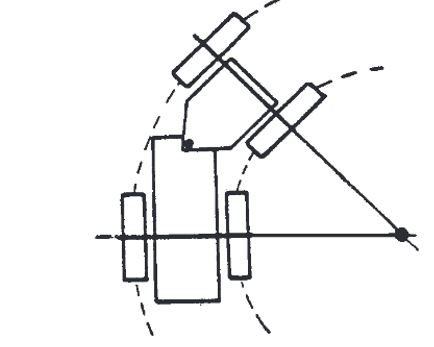
\includegraphics[width=0.5\textwidth]{Images/Knicklenkung.JPG}
\subsection{Achsschenkellenkung}
\begin{itemize}	
\item Die Standfestigkeit wird auch bei vollem Lenkeinschlag nicht beeinträchtigt.\\
\item Heutige zweiachsige PWS und Nutzfahrzeuge sind fast alle mit Achsschenkellenkung gebaut.\\
\item Das kurveninnere Rad ist stärker eingeschlagen als das kurvenäussere.\\
\end{itemize}
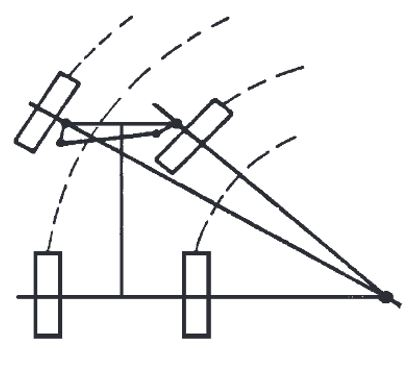
\includegraphics[width=0.5\textwidth]{Images/Achsschellenlenkung.JPG}
\subsubsection{Lenktrapez}
\begin{itemize}
\item Ermöglicht unterschiedliche Einschlagwinkel der Vorderräder.\\
\item Ermöglicht einfaches einstellen eines Spurwinkels.\\
\item Zur Berechnung von Lenktrapezen gibt es vorgefertigte EXEL Tabellen im Web.\\
\end{itemize}
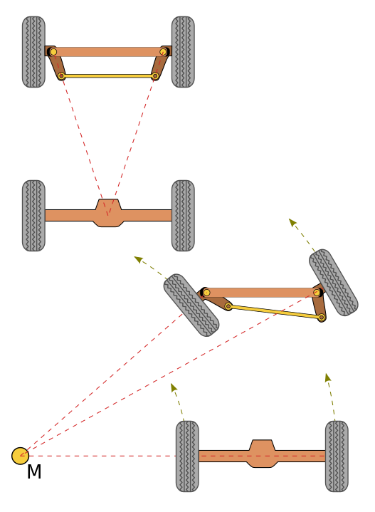
\includegraphics[width=0.5\textwidth]{Images/Lenktrapez.png}
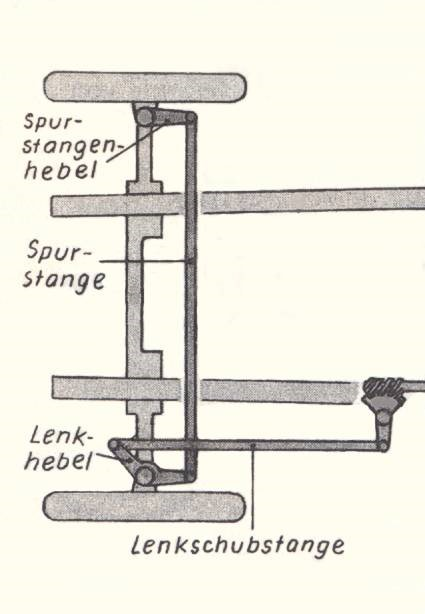
\includegraphics[width=0.5\textwidth]{Images/Lenktrapez2.jpg}
\subsection{Zweiradlenkung}
\begin{itemize}	
\item Lenkung mit einem Zwei- oder Dreiradfahrzeug durch unterschiedlich schnell rotierende Räder.\\
\end{itemize}
\subsection{Lenkung für Kettenfahrzeuge}
\begin{itemize}	
\item Die Lenkung kann durch unterschiedlich schnelles laufen lassen der Ketten realisiert werden.\\
\end{itemize}